\documentclass[aps,prb,onecolumn,nofootinbib,superscriptaddress]{revtex4-2}
\usepackage{amsmath,amssymb,amsthm,mathtools,bm}
\usepackage{booktabs}
\usepackage[colorlinks=true,linkcolor=blue,citecolor=blue,urlcolor=blue]{hyperref}
\usepackage{microtype}
\usepackage{graphicx}
\hypersetup{pdftitle={Finite-range overcomplete Wannier measurements and bulk topology},pdfauthor={Asadullah Bhuiyan}}
\newcommand{\id}{\mathbf{1}}
\newcommand{\tr}{\operatorname{tr}}
\newcommand{\Tr}{\operatorname{Tr}}
\newcommand{\Ch}{\mathfrak C}
\newcommand{\bk}{\boldsymbol k}
\newcommand{\br}{\boldsymbol r}
\newcommand{\bd}{\boldsymbol d}
\newcommand{\bq}{\boldsymbol q}
\newcommand{\rec}{\boldsymbol m}
\newcommand{\ket}[1]{\lvert#1\rangle}
\newcommand{\bra}[1]{\langle#1\rvert}
\newcommand{\kett}[1]{\lvert#1\rangle\!\rangle}
\newcommand{\brr}[1]{\langle\!\langle#1\rvert}
\newcommand{\intk}{\int_{\mathrm{BZ}}\frac{d^2k}{(2\pi)^2}}
\newcommand{\intq}{\int_{\mathrm{BZ}}\frac{d^2q}{(2\pi)^2}}
\begin{document}
\title{Finite-range overcomplete Wannier measurements and bulk topology}
\author{Asadullah Bhuiyan}
\noaffiliation
\date{October 6, 2026}
\begin{abstract}
Overcomplete Wannier modes provide a local description of the occupations of a
Chern band, but their exact spatial tails cannot be retained in a finite-range
circuit. We explain what changes when these modes are truncated. Starting from
the exact occupied projector, we derive the effective form factors and the
auxiliary Hamiltonian built from the truncated modes. We then give two sufficient
conditions under which band mixing preserves the reference Chern number and
evaluate the shortest nontrivial square window in the model used for adaptive
preparation. The onsite limit provides a useful contrast: an overlap zero can
survive even though the auxiliary band is trivial. Finally, we distinguish these
reference-state results from the topology of states produced by conditioned
measurements, including trajectories whose particle number changes.
\end{abstract}
\maketitle
\setcounter{tocdepth}{2}
\tableofcontents

\section{The ideal construction}
\label{sec:ideal}

The adaptive circuit fills modes associated with the lower band and empties
modes associated with the upper band. With exact overcomplete Wannier (OW)
functions, these conditions select the intended Chern insulator. With truncated
functions, the two sets of conditions are no longer generally compatible. The
question is whether losing exact stabilization also requires losing the bulk
topology. To address this question, we first identify the state that the
untruncated construction is designed to prepare, following the projection
construction used in BPJ~\cite{BPJ}.

We consider two orbitals per unit cell and set the lattice spacing to one unless
it is displayed explicitly. The single-particle Hamiltonian and band projectors
are
\begin{equation}
 h(\bk)=\boldsymbol n(\bk)\cdot\boldsymbol\sigma,\qquad
 \boldsymbol n(\bk)=(\sin k_x,\sin k_y,\alpha-\cos k_x-\cos k_y),\qquad
 P_\pm(\bk)=\frac{\id\pm\widehat{\boldsymbol n}(\bk)\cdot\boldsymbol\sigma}{2}.
 \label{eq:model}
\end{equation}
Here $\widehat{\boldsymbol n}=\boldsymbol n/|\boldsymbol n|$ is a unit vector;
the hat does not denote an operator. Our orientation convention assigns
$\Ch[P_-]=1$ for $0<\alpha<2$. The many-body state
$\kett{\mathrm{CI}}$ occupies the lower band and has one fermion per unit cell.

Choose the two orthonormal trial orbitals
$\tau_A=(1,1)^{\mathsf T}/\sqrt2$ and
$\tau_B=(1,-1)^{\mathsf T}/\sqrt2$. In the full single-particle Hilbert space,
write the normalized OW states as
\begin{equation}
 \ket{W_{\br,\nu,\pm}}=
 \frac{P_\pm\ket{\br,\tau_\nu}}{\sqrt{Z_{\nu,\pm}}},\qquad
 Z_{\nu,\pm}=\intk\tau_\nu^\dagger P_\pm(\bk)\tau_\nu=\frac12.
 \label{eq:ow}
\end{equation}
The last equality follows from reflection symmetry: the only Pauli component
seen by either trial orbital is $\sigma^x$, and
$\intk\widehat n_x=0$. The physical orbital index is $\mu$; $\nu=A,B$
labels the two OW families, not two new physical orbitals.

Completeness of the trial orbitals gives a particularly simple reconstruction:
\begin{equation}
 \frac12\sum_{\br,\nu}\ket{W_{\br,\nu,-}}\bra{W_{\br,\nu,-}}
 =P_-\left(\sum_{\br,\nu}\ket{\br,\tau_\nu}\bra{\br,\tau_\nu}\right)P_-
 =P_-^2=P_-.
 \label{eq:tight}
\end{equation}
Thus the lower-band OW modes form a tight frame. The factor $1/2$ compensates
for their redundancy; summing their projectors without this factor gives
$2P_-$, not a physical occupation matrix.

To see the role of the two families, choose a normalized Bloch eigenvector
$\ket{\psi_-(\bk)}$ on a local momentum patch. Its OW form factors are
\begin{equation}
 f_{\nu,-}(\bk)=\sqrt2\,\langle\psi_-(\bk)|\tau_\nu\rangle,
 \qquad \sum_{\nu=A,B}|f_{\nu,-}(\bk)|^2=2.
 \label{eq:two-families}
\end{equation}
An individual form factor has zeros, but the two cannot vanish at the same
momentum. One family supplies the band component missed by the other. The
projector is globally smooth even though a normalized occupied eigenvector
cannot be chosen smooth and periodic everywhere. Projecting local trial
orbitals therefore produces exponentially localized, nonorthogonal modes
without constructing a forbidden orthonormal Wannier basis~\cite{Li2024}.

Let $i=(\br,\mu)$ and $\{\hat c_i,\hat c_j^\dagger\}=\delta_{ij}$.
The mode operator is $\hat\chi_j=\sum_i W_j(i)^*\hat c_i$, where $j$ collects
the center, family, and band labels. Its number operator
$\hat N_j=\hat\chi_j^\dagger\hat\chi_j$ is a projector. The target satisfies
\begin{equation}
 \hat N_{\br,\nu,-}\kett{\mathrm{CI}}=\kett{\mathrm{CI}},\qquad
 (\hat{\mathbf{1}}-\hat N_{\br,\nu,+})\kett{\mathrm{CI}}=\kett{\mathrm{CI}}.
 \label{eq:stabilizers}
\end{equation}
Distinct OW number operators need not commute. Nevertheless, these exact
conditions are compatible because the two families span the occupied band,
while all upper-band modes are orthogonal to it.

We will distinguish the modes defining the operations from the state on which
they act. In BPJ notation the latter has correlation matrix
\begin{equation}
 (G_{\rec})_{ij}=\Tr(\hat\rho_{\rec}\hat c_i^\dagger\hat c_j),
 \qquad \Gamma_{\rec}=G_{\rec}^{\mathsf T},\qquad
 \Gamma_{\rec}^2=\Gamma_{\rec}
 \label{eq:trajectory}
\end{equation}
for a pure number-conserving Gaussian trajectory with measurement record
$\rec$. The transpose converts to the single-particle projector ordering.
For the ideal target $\Gamma=P_-$. A typical conditioned state need not be
translation invariant, so it need not have a rank-one occupied band at each
momentum. Nor is the record average $\overline\Gamma$ generally a projector.

\section{What a finite window changes}
\label{sec:window}

We now truncate the OW wavefunction rather than its outer product. Define
\begin{equation}
 P_-(\bd)=\intk e^{i\bk\cdot\bd}P_-(\bk),\qquad
 g_w(\bd)=\begin{cases}1,&|d_x|,|d_y|\le w,\\0,&\text{otherwise},\end{cases}
 \qquad w=n_{\rm shell}.
 \label{eq:fourier}
\end{equation}
With this convention $P_-(\bk)=\sum_{\bd}e^{-i\bk\cdot\bd}P_-(\bd)$.
An OW mode centered at $\br$ has coefficients proportional to
$P_-(\br'-\br)\tau_\nu$. Its truncated, normalized Fourier amplitude is
\begin{equation}
 W_{\nu,-;w}(\bk)=\frac{F_w(\bk)\tau_\nu}{\sqrt{Z_{\nu,-;w}}},\qquad
 F_w(\bk)=\sum_{\bd}g_w(\bd)P_-(\bd)e^{-i\bk\cdot\bd},\qquad
 Z_{\nu,-;w}=\sum_{\bd}g_w(\bd)^2\|P_-(\bd)\tau_\nu\|^2.
 \label{eq:truncated}
\end{equation}
The normalization is in real space, equivalently
$\intk\|W_{\nu,-;w}(\bk)\|^2=1$. It is not a normalization separately at
each momentum. At finite $w$, $F_w$ need not be a projector.
The amplitude of a translated mode acquires only the phase
$e^{-i\bk\cdot\br}$; we set its center to zero below.

\subsection{The effective overlap and opposite-band weight}

Substituting the Fourier representation of $P_-(\bd)$ into
Eq.~\eqref{eq:truncated} gives
\begin{equation}
 F_w(\bk)=\intq\widetilde g_w(\bk-\bq)P_-(\bq),\qquad
 \widetilde g_w(\bq)=D_w(q_x)D_w(q_y),\qquad
 D_w(q)=\sum_{d=-w}^{w}e^{-iqd}.
 \label{eq:convolution}
\end{equation}
Projecting the truncated mode back onto the target lower band then yields
\begin{equation}
 f^{(w)}_{\nu,-}(\bk)
 =\langle\psi_-(\bk)|W_{\nu,-;w}(\bk)\rangle
 =\frac{1}{\sqrt{Z_{\nu,-;w}}}\intq\widetilde g_w(\bk-\bq)
 \langle\psi_-(\bk)|\psi_-(\bq)\rangle
 \langle\psi_-(\bq)|\tau_\nu\rangle.
 \label{eq:feff}
\end{equation}
This is a convolution dressed by the overlap of Bloch states at different
momenta. The product inside the integral is well defined even when several
momentum patches are required. A change of gauge at $\bq$ cancels between its
two factors; a change of gauge at $\bk$ changes only the phase of the resulting
overlap. On a finite periodic lattice, each normalized momentum integral is
replaced by $N_{\rm uc}^{-1}\sum_{\bk}$.

There is also an upper-band component. If
$b^{(w)}_\nu=\langle\psi_+|W_{\nu,-;w}\rangle$, completeness gives
\begin{equation}
 \intk|f^{(w)}_{\nu,-}|^2+\intk|b^{(w)}_\nu|^2=1.
 \label{eq:leakage}
\end{equation}
Thus truncation changes both the in-band form factor and the band content of
the measurement mode. The first term need no longer integrate to one. In
particular, renormalizing the effective overlap by itself would conceal part
of the opposite-band weight. Figure~\ref{fig:mode} keeps the real-space
normalization of Eq.~\eqref{eq:truncated}.

\subsection{What an overlap zero tells us}

The phase of $f^{(w)}_{\nu,-}$ must be studied in a smooth local gauge. On a
disk $D$ containing an isolated zero and no gauge singularity, define its
boundary winding by
\begin{equation}
 \nu_D[f]=\frac{1}{2\pi}\oint_{\partial D}d\arg f.
 \label{eq:winding}
\end{equation}
Suppose the untruncated and truncated overlaps are compared in the same local
gauge and
$\max_{\partial D}|f^{(w)}-f|<\min_{\partial D}|f|$.
Then $(1-s)f+sf^{(w)}$ never vanishes on $\partial D$. Its winding is an
integer continuous in $s$, and hence is unchanged. This preserves the total
signed index of the enclosed zeros, not necessarily their number or position.
No assumption of complex analyticity in $k_x+ik_y$ is needed.

The local statement should not be confused with a globally periodic scalar
winding argument. Under a Bloch gauge change, $f^{(w)}$ transforms with the
inverse phase of the target eigenvector. Equivalently,
$P_-W_{\nu,-;w}$ is a section of the target band. If it were nonzero
everywhere, its normalization would trivialize that band. A nontrivial target
therefore still requires a zero somewhere, provided this projected section
is not identically zero. Truncation can displace the original zero without
removing the target-band obstruction.

By contrast, if the full two-component field $W_{\nu,-;w}(\bk)$ is nowhere
zero, then
$W_{\nu,-;w}/\|W_{\nu,-;w}\|$ is a global smooth periodic section of
\emph{its own} line bundle, whose Chern number is zero. The overlap zero is
then a statement about its relation to the target, not a nonzero Chern number
carried by this single compact-support mode. We will see this distinction
explicitly already for $w=0$.

\subsection{Spatial extent and discarded weight}

Two elementary measures of the exact normalized mode are
\begin{equation}
 \xi_{\rm rms}^2=\sum_{\bd}|\bd|^2\|W_{\nu,-}(\bd)\|^2,
 \qquad p_w=\sum_{\bd}g_w(\bd)\|W_{\nu,-}(\bd)\|^2=2Z_{\nu,-;w}.
 \label{eq:weight}
\end{equation}
Here the RMS radius is measured about the nominal trial-orbital cell, not
about the probability centroid. At $\alpha=1$ we find
$\xi_{\rm rms}\simeq0.673521a$, while $p_1\simeq0.992155$ and
$p_2\simeq0.999137$. The $A$-family centroid is
$\langle\br\rangle\simeq(0,-0.185336)a$, giving a centered RMS spread
of $0.647520a$. The axial asymptotic tail is controlled instead by the
nearest complex-momentum singularity. Here
$|\boldsymbol n|^2=3-2\cos k_x-2\cos k_y+2\cos k_x\cos k_y$.
Putting $k_x=i\kappa$ and $k_y=\pi$ gives
$5-4\cosh\kappa=0$, hence the axial decay length
$\xi_{{\rm exp},x}=a/\log2\simeq1.442695a$.
This tail scale is not the RMS radius and is not an isotropic bound on every
direction. A long asymptotic tail can carry very little total weight.

The spread of a band-projected state also depends on quantum geometry.
For a normalized amplitude $a(\bk)$ multiplying a local Bloch state, direct
differentiation and Parseval's identity give
\begin{equation}
 \langle\br^2\rangle
 =\intk\left[|(-i\boldsymbol\nabla_{\bk}-\boldsymbol{\mathcal A})a|^2
              +\tr g(\bk)|a|^2\right],\qquad
 \mathcal A_\mu=i\langle\psi_-|\partial_\mu\psi_-\rangle,
 \quad g_{\mu\nu}=\operatorname{Re}\langle\partial_\mu\psi_-|
 (\id-P_-)|\partial_\nu\psi_-\rangle.
 \label{eq:spread}
\end{equation}
The patch transformations of $a$ and $\boldsymbol{\mathcal A}$ make this
expression gauge invariant. Minimizing it is a geometry-dependent spectral
problem for $(-i\boldsymbol\nabla-\boldsymbol{\mathcal A})^2+\tr g$,
acting on amplitudes with the appropriate patch transitions, as developed
by Li \emph{et al.}~\cite{Li2024}. The geometric data
cannot in general be replaced by the Chern number alone. In particular, a
spread bound derived for homogeneous ideal geometry is not a universal
minimum truncation radius for our lattice model. We use the directly computed
$p_w$ and projector errors instead.

\begin{figure}[t]
 \centering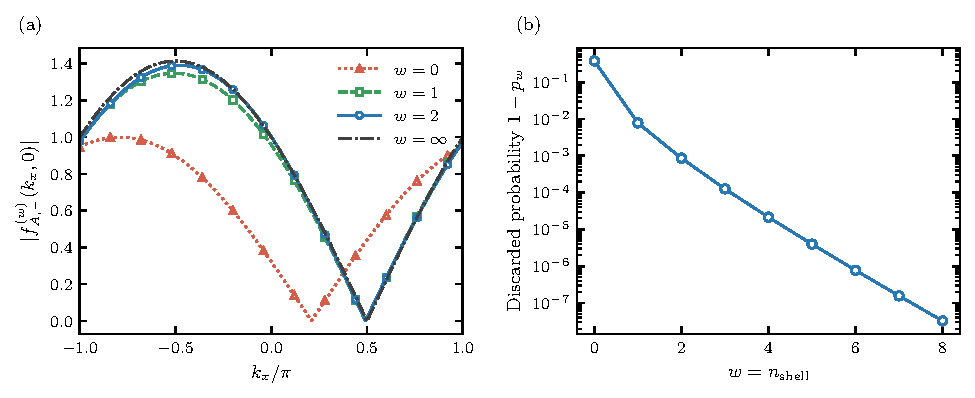
\includegraphics[width=6.5in]{figures/ow_mode_truncation.pdf}
 \caption{\textbf{Effect of truncating an OW mode.} (a) Lower-band overlap
 of the $A$-family mode along $k_y=0$ at $\alpha=1$, with unit real-space
 norm for each mode. (b) Probability discarded by the square window.
 The form-factor zero moves under truncation even when most weight is retained.
 These are deterministic band calculations, not trajectory averages.}
 \label{fig:mode}
\end{figure}

\section{The auxiliary Hamiltonian of the truncated modes}
\label{sec:auxiliary}

To compare an occupied band with the target, we must combine the measurement
modes before taking a spectral projection. The relevant translation-summed
frame operators are
\begin{equation}
 S_{\pm,w}(\bk)=\sum_{\nu=A,B}W_{\nu,\pm;w}(\bk)
 W_{\nu,\pm;w}^\dagger(\bk).
 \label{eq:frames}
\end{equation}
For clarity, a single centered mode $W(\bd)$ has an outer product with two
independent Fourier sums:
\begin{equation}
 W(\bk)W^\dagger(\bk')
 =\sum_{\bd,\bd'}e^{-i\bk\cdot\bd}e^{i\bk'\cdot\bd'}
 W(\bd)W^\dagger(\bd').
 \label{eq:both-indices}
\end{equation}
With normalized finite-volume momentum kets, its matrix element has an
additional factor $N_{\rm uc}^{-1}$. Summing over all translated centers
produces $N_{\rm uc}\delta_{\bk,\bk'}$, yielding Eq.~\eqref{eq:frames}.
For one normalized untruncated family $W$, the corresponding real-space
kernel is an autocorrelation,
\begin{equation}
 S_w(\bd)=\frac1{p_w}\sum_{\boldsymbol x}g_w(\boldsymbol x+\bd)g_w(\boldsymbol x)
 W(\boldsymbol x+\bd)W^\dagger(\boldsymbol x),
 \label{eq:autocorrelation}
\end{equation}
where $p_w$ is its retained probability. Both window factors are necessary.
For one wavefunction family its range can reach $2w$; it is not obtained by
simply multiplying the original frame kernel by $g_w(\bd)$.

Since $g_w(0)=1$, the truncated upper-band amplitude is
$(\id-F_w)\tau_\nu/\sqrt{Z_{\nu,+;w}}$. For a real inversion-symmetric
window, $F_w^\dagger=F_w$. Keeping potentially unequal normalizations gives
\begin{equation}
 S_{-,w}=F_wD_{-,w}F_w^\dagger,\qquad
 S_{+,w}=(\id-F_w)D_{+,w}(\id-F_w)^\dagger,\qquad
 D_{\pm,w}=\sum_\nu\frac{\tau_\nu\tau_\nu^\dagger}{Z_{\nu,\pm;w}}.
 \label{eq:general-frame}
\end{equation}
This is the appropriate expression if the window or trial orbitals break the
normalization symmetry.

For the square window in Eq.~\eqref{eq:fourier}, write
$F_w=(\id-\boldsymbol d_w\cdot\boldsymbol\sigma)/2$.
The trace is one because the trace of $P_-(\bd)$ is $\delta_{\bd,0}$.
The four norms are equal: reflection makes $\intk d_{w,x}=0$, while
$\tau_{A,B}$ have zero $\sigma^{y,z}$ expectation values. Consequently,
\begin{equation}
 Z_{\nu,\pm;w}=Z_w=\frac{1+\intk|\boldsymbol d_w|^2}{4},\qquad
 S_{-,w}=\frac{F_w^2}{Z_w},\qquad
 S_{+,w}=\frac{(\id-F_w)^2}{Z_w}.
 \label{eq:symmetric-frame}
\end{equation}
We define the signed auxiliary Hamiltonian and its occupied projector by
\begin{equation}
 h_w=S_{+,w}-S_{-,w}=\frac{\id-2F_w}{Z_w},\qquad
 R_w=\mathbf{1}_{(-\infty,0)}(h_w)=\mathbf{1}_{(1/2,\infty)}(F_w),
 \label{eq:hw}
\end{equation}
whenever the cutoff is gapped. The simplification of $h_w$ follows from
cancellation of the quadratic terms; it does not replace the two-index
Fourier transform by a one-index transform. It is special to the equal-norm
construction. In the untruncated limit $Z_\infty=1/2$, $h_\infty=2(\id-2P_-)$,
and $R_\infty=P_-$.

This construction also explains why a finite-range auxiliary Hamiltonian can
have a nontrivial band. Its spectral projection $R_w$ is nonlinear in $F_w$
and generally has exponential spatial tails, even though $h_w$ has finite
range. It is not a compactly supported spanning set for the occupied band.
The compact-support obstruction of Dubail and Read therefore does not forbid
such a Hamiltonian: redundancy alone cannot provide compact modes confined
to and spanning an exact nontrivial band, but our truncated modes leak out
of that band~\cite{DubailRead2015}. The objects $F_w$, $S_{\pm,w}$, and $R_w$
must not be identified with one another.

\section{Why band mixing can preserve topology}
\label{sec:stability}

For a smooth periodic occupied projector $P(\bk)$, we use
\begin{equation}
 \Ch[P]=\frac{1}{2\pi i}\int_{\mathrm{BZ}}d^2k\,
 \tr\bigl(P[\partial_{k_x}P,\partial_{k_y}P]\bigr).
 \label{eq:chern}
\end{equation}
Its integer character can be seen by choosing local occupied eigenvectors.
On an overlap they differ by a phase $e^{i\theta}$, so the connection
one-forms $\langle\psi|d\psi\rangle$ differ by $i\,d\theta$.
Stokes' theorem reduces the integrated curvature to integer
transition-function windings. The same expression is continuous under a
smooth fixed-rank deformation. An integer cannot vary continuously, so the
Chern number is constant along such a path~\cite{Avron1983}. We next give two
ways to construct the required path; neither assumes a global eigenvector.

\subsection{A nonzero overlap is sufficient}

Let $P$ and $R$ be smooth periodic rank-one projectors. Locally, write an
occupied vector of $R$ as
$\ket v=a\ket{\psi_-}+b\ket{\psi_+}$, with
$|a|^2+|b|^2=1$, and set $P=P_-$.
The target overlap and opposite-band weight are
\begin{equation}
 \tr(PR)=|a|^2=1-\eta,\qquad
 \eta=\tr[(\id-P)R]=|b|^2.
 \label{eq:eta}
\end{equation}
If $\tr(PR)>0$ at every momentum, the upper-band component can be removed
continuously:
\begin{equation}
 B_s=P+(1-s)(\id-P),\qquad
 R_s=\frac{B_sRB_s}{\tr(B_sRB_s)},\qquad
 \tr(B_sRB_s)=1-\eta+(1-s)^2\eta>0.
 \label{eq:overlap-path}
\end{equation}
The numerator has rank one and is positive, so division by its trace makes
it an orthogonal projector. Moreover, $R_0=R$ and
$PRP=\tr(PR)P$ implies $R_1=P$. Compactness of the Brillouin torus makes
the positive overlap uniformly bounded away from zero. Thus
\begin{equation}
 \tr[P(\bk)R(\bk)]>0\text{ for every }\bk
 \quad\Longrightarrow\quad \Ch[R]=\Ch[P].
 \label{eq:overlap-result}
\end{equation}
The physical point is that a coherent admixture of the other band need not
change the topology of the occupied line. Different Chern numbers require
an orthogonality point, although an orthogonality point alone does not imply
different topology. An average bound on $\eta$ would not suffice: it can
miss a small region where $|a|$ vanishes. For several occupied bands, the
overlap map must instead have full rank everywhere.

A related distinction appears after coherent quenches: a state's Chern
number can remain unchanged even though it is not the ground state of the
post-quench Hamiltonian~\cite{Caio2015}. The nonequilibrium Hall response is
another quantity and need not be quantized~\cite{Caio2016}.

\subsection{A controlled truncation keeps the auxiliary gap open}

For our auxiliary band, a convenient sufficient condition is
\begin{equation}
 \delta_w=\sup_{\bk}\|F_w(\bk)-P_-(\bk)\|_{\rm op}<\frac12.
 \label{eq:delta}
\end{equation}
Consider $F_{w,s}=P_-+s(F_w-P_-)$ and the unnormalized Hamiltonian
$H_{w,s}=\id-2F_{w,s}$. Each eigenvalue of $F_{w,s}$ lies within
$s\delta_w$ of either zero or one. The two intervals do not reach $1/2$,
and hence
\begin{equation}
 \min_{\bk,n}|E_n[H_{w,s}(\bk)]|\ge1-2s\delta_w>0.
 \label{eq:gap-bound}
\end{equation}
The spectral projector above $1/2$ supplies the required smooth fixed-rank
path from $P_-$ to $R_w$. At the endpoint $h_w=H_{w,1}/Z_w$ differs only
by a positive scale. We obtain
\begin{equation}
 \delta_w<\frac12\quad\Longrightarrow\quad
 \Ch[R_w]=1,\qquad
 \min_{\bk,n}|E_n[h_w]|\ge\frac{1-2\delta_w}{Z_w}.
 \label{eq:bound-result}
\end{equation}
For the traceless two-band Hamiltonian, the full separation between the
bands is twice this minimum absolute energy.

At a fixed gapped $\alpha$, the projector kernel decays exponentially.
For the indicator window,
\begin{equation}
 \delta_w\le\sum_{\bd\notin[-w,w]^2}\|P_-(\bd)\|_{\rm op}
 \longrightarrow0\qquad(w\longrightarrow\infty).
 \label{eq:tail}
\end{equation}
This bound is independent of the volume and proves stability for sufficiently
large finite windows. It does not by itself certify $w=1$, nor a range uniform
through a target gap closing. If the normalization symmetry is absent, one
can apply the same spectral argument directly to $h_w-h_\infty$, bounding
its uniform operator norm by the distance of the untruncated spectrum from
zero. Appendix~\ref{app:synthesis} gives an alternative estimate from the
normalized mode errors.

The retained probability $p_w$ is a useful local diagnostic but is weaker
than Eq.~\eqref{eq:delta}. It integrates information over momenta, whereas
the gap must remain open everywhere. Likewise, two projectors can be close
on average without satisfying the pointwise overlap criterion. These
distinctions matter when interpreting a very small measured band leakage.

\section{Range one and the onsite counterexample}
\label{sec:examples}

We evaluate the square-window construction at $\alpha=1$. The Fourier
coefficients are computed on $1024^2$ and $2048^2$ grids; matrix extrema are
then sampled on independent $201^2$ and $401^2$ momentum grids. Table~\ref{tab:checks}
reports the highest-resolution values. The zero is refined on $k_y=0$ in a
smooth local frame, rather than identified with the smallest sampled value
on a momentum grid. Loops of several radii and resolutions give winding
$-1$ around each listed zero.

\begin{table}[t]
 \caption{\textbf{Square-window checks at $\alpha=1$.} The effective overlap
 uses the normalized $A$-family mode. $k_*$ lies on $k_y=0$. The last three
 columns are sampled extrema: they are not rigorous continuum bounds.
 $E_{\min}$ is the minimum absolute energy of the normalized $h_w$, not the
 full band separation.}
 \label{tab:checks}
 \begin{ruledtabular}
 \begin{tabular}{cccccc}
 $w$ & $p_w$ & $k_*/\pi$ & $\delta_w^{\rm grid}$ & $\min\tr(P_-R_w)$ & $E_{\min}^{\rm grid}$\\
 \hline
 0 & 0.620624 & 0.209346 & 0.745585 & 0.000000 & 1.582825 \\
1 & 0.992155 & 0.492186 & 0.098754 & 0.990190 & 1.802426 \\
2 & 0.999137 & 0.492488 & 0.033797 & 0.999004 & 1.902788 \\

 \end{tabular}
 \end{ruledtabular}
\end{table}

For $w=1$, more than $99\%$ of the mode's probability is retained, the
sampled error is approximately $0.09875$, and the minimum sampled target
overlap exceeds $0.9901$. Independently summing the four normalized mode
outer products reproduces Eq.~\eqref{eq:hw} to numerical precision.
Figure~\ref{fig:band} displays the interpolating spectral separation and
the small but nonuniform mismatch of its occupied band with the target.
These tests give substantial numerical evidence that the shortest nontrivial
square window lies well within the stable reference phase. Fourier quadrature
and finite momentum sampling do not, however, provide an interval-certified
bound on the continuum supremum.

The onsite limit is qualitatively different. Here $w=0$ retains one unit
cell with its two physical orbitals. Reflection symmetry gives
\begin{equation}
 F_0=\intk P_-(\bk)=\frac{\id-d_0\sigma^z}{2},\qquad
 d_0=\intk\widehat n_z\simeq0.491169,
 \qquad Z_0=\frac{1+d_0^2}{4}.
 \label{eq:onsite}
\end{equation}
Therefore $h_0=(d_0/Z_0)\sigma^z$ and
$R_0=\ket{\downarrow}\bra{\downarrow}$ is constant, so
$\Ch[R_0]=0$. The onsite auxiliary Hamiltonian is gapped but trivial.
At $\bk=0$, the target projector is instead
$P_-(0)=\ket{\uparrow}\bra{\uparrow}$. Its overlap with $R_0$ vanishes,
and the interpolation has
\begin{equation}
 F_{0,s}(0)=
 \begin{pmatrix}1-s(1+d_0)/2&0\\0&s(1+d_0)/2\end{pmatrix},
 \qquad s_*=\frac1{1+d_0},\qquad H_{0,s_*}(0)=0.
 \label{eq:crossing}
\end{equation}
The failure is not just that a sufficient estimate becomes inconclusive:
this particular path actually closes its gap.

Nevertheless, the \emph{mode} $F_0\tau_A/\sqrt{Z_0}$ still has an overlap
zero with the target. On $k_y=0$, a smooth target eigenvector gives
\begin{equation}
 f^{(0)}_{A,-}(k_x,0)=
 \frac{(1-d_0)\cos(k_x/2)-(1+d_0)\sin(k_x/2)}{2\sqrt{2Z_0}},\qquad
 \tan\frac{k_*}{2}=\frac{1-d_0}{1+d_0}.
 \label{eq:onsite-overlap}
\end{equation}
Thus $k_*/\pi\simeq0.2093$, even though the auxiliary band has Chern number
zero. This zero is required by comparing a nonzero global mode with the
nontrivial target bundle; it is not evidence that onsite measurements
prepare a Chern insulator. It illustrates why survival of overlap winding
and stability of the auxiliary occupied band are different statements.

\begin{figure}[t]
 \centering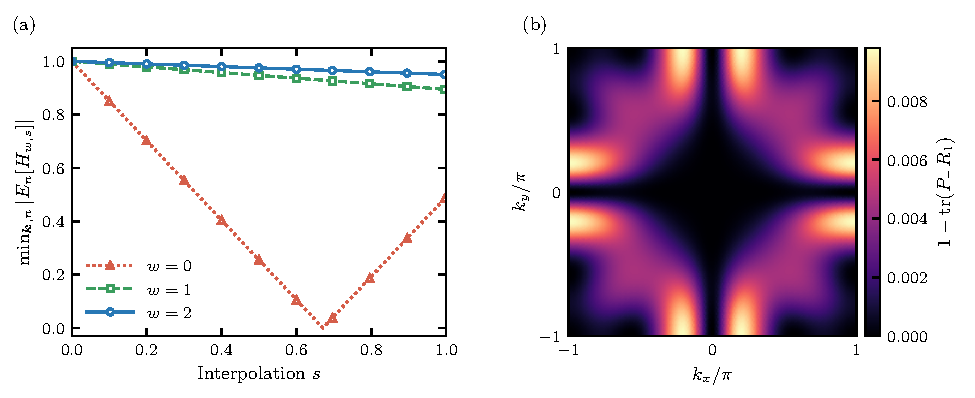
\includegraphics[width=6.5in]{figures/auxiliary_band_stability.pdf}
 \caption{\textbf{Auxiliary-band stability.} (a) Minimum absolute energy of
 $H_{w,s}=\mathbf{1}-2[(1-s)P_-+sF_w]$ along the interpolation. The onsite
 path closes at $s_*=1/(1+d_0)$; the $w=1,2$ paths remain gapped on the
 sampled momentum grid. (b) Target-band mismatch $1-\tr(P_-R_1)$ at
 $\alpha=1$. The positive normalization $1/Z_w$ is omitted in (a).
 These quantities characterize auxiliary bands, not stochastic trajectories.}
 \label{fig:band}
\end{figure}

\section{From reference states to conditioned dynamics}
\label{sec:dynamics}

The auxiliary Hamiltonian gives a natural reference state, but it is not
automatically the generator of the circuit. We can make the connection and
its limitation explicit. For normalized truncated modes define the penalties
\begin{equation}
 \hat q_{j,-}=\hat{\mathbf{1}}-\hat N_{j,-},\qquad
 \hat q_{j,+}=\hat N_{j,+},\qquad
 \hat H_{\rm pen}=\sum_{j,n=\pm}\hat q_{j,n}.
 \label{eq:penalties}
\end{equation}
Apart from a many-body constant, its one-body matrix is exactly
$S_{+,w}-S_{-,w}=h_w$. Because each $\hat q$ is a projector,
\begin{equation}
 e^{-\lambda\hat q}=\hat{\mathbf{1}}+(e^{-\lambda}-1)\hat q,
 \qquad e^{-\lambda\hat q_{j,-}}\xrightarrow{\lambda\to\infty}\hat N_{j,-},
 \qquad e^{-\lambda\hat q_{j,+}}\xrightarrow{\lambda\to\infty}
 \hat{\mathbf{1}}-\hat N_{j,+}.
 \label{eq:filter}
\end{equation}
These are the desired-outcome branches without correction. At fixed finite
volume and $\beta$, weak filters obey the Trotter limit
\begin{equation}
 e^{-\beta\hat H_{\rm pen}}
 =\lim_{M\to\infty}\left(\prod_{j,n}e^{-\beta\hat q_{j,n}/M}\right)^M.
 \label{eq:trotter}
\end{equation}
Within the half-filled sector, normalized imaginary-time evolution selects
the ground state of $h_w$ if the initial state has nonzero overlap with it
and that ground state is unique. This conclusion does not apply to an
initial state in the wrong number sector.

Taking each filter to be a strong projector at fixed step size is a
different limit. The penalties do not commute, so Eq.~\eqref{eq:trotter}
does not identify the strong-filter circuit with imaginary time. Further,
actual records include undesired outcomes followed by correction. In the
ideal fresh-ancilla protocol, filling and depletion introduce physical-layer
creation and annihilation branches. An earlier corrected mode can then be
disturbed by a later, nonorthogonal one. At finite range there is generally
no common state that fills every lower-family mode and empties every
upper-family mode.

This distinction also separates conditional dynamics from dissipative
preparation of a unique pure state. Goldstein's no-go theorem and constructions
concern Gaussian Lindblad preparation under specified locality and convergence
conditions~\cite{Goldstein2019}. They do not identify our auxiliary ground
state with every conditioned output. Likewise, the untruncated Markovian
analysis in BPJ Appendix D is not a proof of stability of all finite-range
records~\cite{BPJ}.

\subsection{Particle addition and removal}

Charge fluctuations do not invalidate the question of a bulk invariant, but
they prevent a direct equal-rank comparison. To see this, take a pure Slater
state with projector $\Gamma$ and apply
$\hat c^\dagger(v)=\sum_i v_i\hat c_i^\dagger$.
Writing the state as an exterior product of occupied orbitals shows that
the component $\Gamma v$ gives zero by Pauli exclusion. For a nonzero-probability
event the surviving orbital and new projector are
\begin{equation}
 \phi_+=\frac{(\id-\Gamma)v}{\sqrt{v^\dagger(\id-\Gamma)v}},\qquad
 \Gamma'=\Gamma+\phi_+\phi_+^\dagger.
 \label{eq:gain}
\end{equation}
Similarly, choose an occupied basis whose first vector is proportional to
$\Gamma v$. Annihilation removes precisely that vector, yielding
\begin{equation}
 \phi_-=\frac{\Gamma v}{\sqrt{v^\dagger\Gamma v}},\qquad
 \Gamma'=\Gamma-\phi_-\phi_-^\dagger.
 \label{eq:loss}
\end{equation}
Both changes have operator norm one and change
$N_F=\tr\Gamma$ by one. A small \emph{relative} number change therefore does
not imply that the occupied projector is a small operator-norm perturbation.

If $v$ is supported near one point and $\Gamma_{ij}$ decays rapidly in the
bulk, the numerators in Eqs.~\eqref{eq:gain}--\eqref{eq:loss} inherit that
locality. For a fixed allowed event the denominator is nonzero. A finite
number of such localized changes is compatible with an unchanged
thermodynamic bulk index: the associated change of the Fredholm operator
is compact, so its index is stable when the locality assumptions defining
that index remain satisfied~\cite{Bellissard1994}. A finite-region Chern
estimator can still change near the modified orbitals.

This reasoning is not uniform over arbitrary long records. Small outcome
probabilities and repeated updates can invalidate uniform locality bounds;
an increasing density of modifications is not a single fixed finite-rank
perturbation in the thermodynamic limit. Net charge also does not count
compensating particle--hole changes. For a reference projector $R$, the
occupation mismatches obey
\begin{equation}
 N_{\rm p}=\tr[(\id-R)\Gamma],\qquad
 N_{\rm h}=\tr[R(\id-\Gamma)],\qquad
 N_{\rm p}-N_{\rm h}=\tr\Gamma-\tr R,\qquad
 N_{\rm p}+N_{\rm h}=\tr(\Gamma-R)^2.
 \label{eq:mismatches}
\end{equation}
The sum can be appreciable even when the difference is zero. Moreover,
these are occupations relative to a chosen reference, not automatically
localized defects or evidence of topological failure.

\subsection{What the present results establish}

The deterministic conclusion is that finite-range truncation need not
destroy the topology of the auxiliary occupied band. We have an explicit
sufficient condition and numerical checks of that condition for the shortest
nontrivial square window. What remains is to control the projectors actually
produced by the circuit, including their spatial decay and the long-time and
large-system limits. Neither a small integrated leakage nor a relaxation
statement for an averaged channel supplies this missing control.

Our existing trajectory-resolved data address a complementary question.
At cycle 40, the deviation $|\overline{C_G}-1|$ decreases from approximately
$2.4\times10^{-3}$ for $L=20$ to $1.4\times10^{-5}$ for $L=40$, using
square hard-wall systems, $100$ trajectories, $w=1$, and disk radius $0.2L$.
The estimator is evaluated within each trajectory before averaging. This
supports the intended bulk phase on the tested scales, but the comparison
increases both system size and disk radius. A finite disk has finite-radius
corrections and is not an exactly quantized invariant~\cite{Kitaev2006}.
These observations should therefore be presented as dynamical numerical
evidence, independently of the auxiliary-band stability argument.

\appendix
\section{A bound directly from normalized OW errors}
\label{app:synthesis}

It is useful to retain a more general estimate that does not use the
cancellation in Eq.~\eqref{eq:hw}. Let $\mathcal T_0$ have columns
$W_{\br,\nu,-}/\sqrt2$, and let $\mathcal T_w$ have columns
$W_{\br,\nu,-;w}/\sqrt2$, with each truncated mode normalized to one.
The tight-frame identity implies
$\mathcal T_0\mathcal T_0^\dagger=P_-$ and
$\|\mathcal T_0\|_{\rm op}=1$. Defining
$E_w=\mathcal T_w-\mathcal T_0$ and
$\epsilon_w=\|E_w\|_{\rm op}$ gives
\begin{equation}
 \mathcal F_w=\mathcal T_w\mathcal T_w^\dagger=\frac12S_{-,w},\qquad
 \|\mathcal F_w-P_-\|_{\rm op}
 \le2\epsilon_w+\epsilon_w^2.
 \label{eq:synthesis}
\end{equation}
Here $\mathcal F_w$ is a quadratic frame operator; it is not $F_w$.
If $2\epsilon_w+\epsilon_w^2<1/2$, the same spectral argument as in
Sec.~\ref{sec:stability} proves that
$\Pi_w=\mathbf{1}_{(1/2,\infty)}(\mathcal F_w)$ has Chern number one.
This is a lower-family-only reference Hamiltonian
$\id-2\mathcal F_w$, distinct from $h_w$. Their occupied projectors must
not be assumed equal outside a regime where that equality has been checked.

For translation-invariant modes, a bound on $\epsilon_w$ can be made
independent of the volume. Write $W_\nu=W_{0,\nu,-}$, with unit real-space
norm, and set
\begin{equation}
 M_1=\max_\nu\|W_\nu\|_1,\qquad
 a_p=\max_\nu\|(1-g_w)W_\nu\|_p,\qquad
 b_w=a_1+\left[(1-a_2^2)^{-1/2}-1\right]M_1.
 \label{eq:tail-norms}
\end{equation}
The $\ell^1$ norms here sum absolute component values over cells and
orbitals; $\ell^2$ is the ordinary mode norm. For $a_2<1$, subtracting
$W_\nu$ from $g_wW_\nu/\|g_wW_\nu\|_2$ bounds the column's $\ell^1$
error by $b_w$. Fourier transformation bounds each Bloch-column error
by the same number. There are two columns divided by $\sqrt2$, so their
combined Frobenius norm, and hence operator norm, is at most $b_w$.
Consequently,
\begin{equation}
 \epsilon_w=\sup_{\bk}\|E_w(\bk)\|_{\rm op}\le b_w,
 \qquad \epsilon_w<\sqrt{3/2}-1
 \quad\Longrightarrow\quad\Ch[\Pi_w]=1.
 \label{eq:synthesis-result}
\end{equation}
Exponential localization makes $M_1$ finite and $a_{1,2}$ tend to zero.
This supplies a sufficient finite-range result without replacing an operator
bound by a per-column squared-weight estimate. It is intentionally
conservative and is not used to certify the range-one example.

\section{Numerical and source checks}
\label{app:checks}

The accompanying calculation uses the existing repository Bloch-projector
and Fourier helpers without invoking circuit dynamics or their plotting
entry point. It verifies equal mode norms, Hermiticity, idempotency of
$R_w$, and the quadratic frame identity independently. Increasing the
Fourier grid from $1024^2$ to $2048^2$ changes the retained coefficients
by less than $10^{-12}$; matrix identities are checked to $10^{-12}$.
The momentum grids contain the $\Gamma$ point, so the onsite crossing
is also checked directly at its analytic $s_*$. We use the spectral
subspace of $F_w$ above $1/2$, not a normalized column of
$F_w$, when constructing $R_w$.

For the overlap zeros, real roots along $k_y=0$ are refined in a smooth
local eigenvector frame. Their winding is checked with $360$ and $720$
segments on loops of radius $0.01$, $0.02$, and $0.04$, using two distinct
local gauges and explicitly nonzero boundary amplitudes. Auxiliary-band
and single-mode Chern numbers are also compared using the
Fukui--Hatsugai--Suzuki discretization~\cite{Fukui2005} on both momentum
grids. For $w=0,1,2$, the auxiliary values are respectively $0,1,1$,
while the resolved nowhere-zero compact spinors give zero. These checks
guard against confusing a single mode with the auxiliary band and against
assigning topology from an unresolved minimum.

The data receipt records grids, normalizations, residuals, sampled extrema,
and source hashes; the plotted arrays and table are regenerated from the
same calculation. The brief trajectory comparison in Sec.~\ref{sec:dynamics}
is taken from the completed slab-topology study rather than rerun here.
No continuum supremum, asymptotic trajectory convergence, or localization
theorem is certified by these finite-grid checks.

\bibliographystyle{apsrev4-2}
\bibliography{references}
\end{document}
